% extra contents of chap2

\section{热学延伸}

\subsection{理想气体内能公式推导}

如图,气体分子在边长为l的立方体容器内运动、三个方向上的速度均为$v$,假设其与容器壁做弹性碰撞,计算气体压强与分子运动速度的关系。
\begin{figure}[ht!]
    \centering
    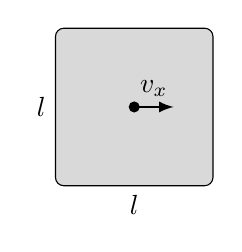
\begin{tikzpicture}
        \filldraw[color=black, fill=gray!30, rounded corners=3pt] (0, 0) rectangle (2, 2);
        \node[below] at (1, 0) {$l$};
        \node[left] at (0, 1) {$l$};
        \draw[thick, -latex] (1, 1) -- node[above] {$v_x$} ++ (0.5, 0) ;
        \fill (1, 1) circle (2pt);
    \end{tikzpicture}
    \caption{气体分子运动与压强}
\end{figure}
由于气体分子在x方向上每折返一次就会与容器壁发生一次碰撞,所以$\Delta t$时间内会与容器壁碰撞$\frac{v\Delta t}{2l}$次。因此这段时间内容器壁受到来自气体分子的冲量为
\begin{equation*}
    2mv\cdot\frac{v_x\Delta t}{2l}=\frac{m{v_x}^2}{l}\Delta t
\end{equation*}
即相当于单个气体分子给予容器壁$F=\frac{m{v_x}^2}{l}$大小的力,相对应的就会有
\begin{equation*}
    P=\frac{F}{l^2}=\frac{m{v_x}^2}{l^3}=\frac{m{v_x}^2}{V}
\end{equation*}
大小的压强。此外,该气体分子也会在y和z方向上做同样的运动,所以其速度的平均值为$\overline{v^2}=\overline{{v_x}^2}+\overline{{v_y}^2}+\overline{{v_z}^2}$。同时,容器内倘若有N个这样的气体分子,那么其压强的总和为
\begin{equation*}
    P=N\cdot\frac{m{v_x}^2}{V}=\frac{Nm\overline{v^2}}{3V}
\end{equation*}
将上述压强值代入理想气体状态方程就可以得到1摩尔该气体分子平均速度的平方。
\begin{gather*}
    PV=nRT\\
    \frac{Nm\overline{v^2}}{3V}V=\frac{N}{N_A}RT\\
    \overline{v^2}=\frac{3RT}{M}
\end{gather*}
那么n摩尔该气体分子的总动能可求。
\begin{equation*}
    n\cdot\frac12M\overline{v^2}=\frac32nRT
\end{equation*}

\subsection{等温变化做功}

\begin{equation*}
    Q_\textrm{吸}=W_\textrm{した}=\int_{V_1}^{V_2}PdV=nRT\cdot\log\frac{V_2}{V_1}
\end{equation*}

\subsection{断热变化PV等式推导}

基于断热变化的热力学第一定律可得
\begin{gather*}
    \Delta U=-W_\textrm{した}\\
    nC_v\Delta T=-PdV
\end{gather*}
简做整理后对两侧分别关于T和V积分
\begin{gather*}
    \int\frac{dT}{T}=-\frac{R}{C_v}\int\frac{dV}{V}\\
    \log T=-\frac{R}{C_v}\log V+c^\prime\\
    T=V^{-\frac{R}{C_v}}\cdot c\\
    TV^{\frac{R}{C_v}}=c
\end{gather*}
在此定义$\gamma=\frac{C_p}{C_v}$,结合$C_p-C_v=R$即有
\begin{equation*}
    TV^{\gamma-1}=c
\end{equation*}
再结合理想气体状态方程就可以得到$PV^\gamma=const$的结论。
